\section{问题背景}

% 第 1–8 页共 480 秒，包含封面与换人过渡。
\begin{frame}
  \pdfbookmark[3]{00:00　开场}{timing-0}
  \titlepage
  \vspace{-6mm}
  \centering
  {\small 冻结图文对比预训练模型（CLIP），在测试时挑选负标签。\\
   哪些词能帮助模型把分布外（OOD）图像与分布内（ID）图像分开？\par}
  \vspace{3mm}
  
\includegraphics[height=1.05cm]{PKU_logo.png}
  \note{25 秒。先给出问题。假设分类器只认识猫和狗，面对盆栽，它为什么不该硬选一个动物？先用八分钟讲论文怎样挑出有用的负标签，再用十一分钟讲我们的正队列、评分与图像实验。}
\end{frame}

\begin{frame}[t,label=paper-start]{为什么图像分类器需要回答“未知”？}
  \pdfbookmark[3]{00:25　已知类别与未知图像}{timing-25}
  假设一款相册只提供“猫”和“狗”两个标签，用户却可以上传任何照片。
  \par\vspace{3mm}
  \begin{columns}[T,onlytextwidth]
    \begin{column}{.48\linewidth}\centering
      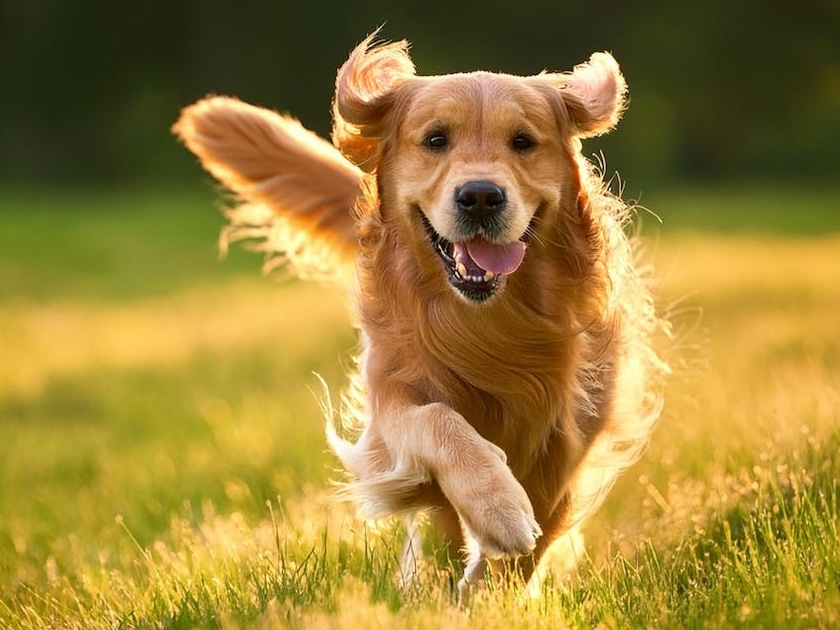
\includegraphics[height=3.05cm]{dog.jpg}\\[1.4mm]
      \accenttext{分布内图像}\\[.6mm]
      \small 狗属于已知类别，可以标为“狗”。
    \end{column}
    \begin{column}{.48\linewidth}\centering
      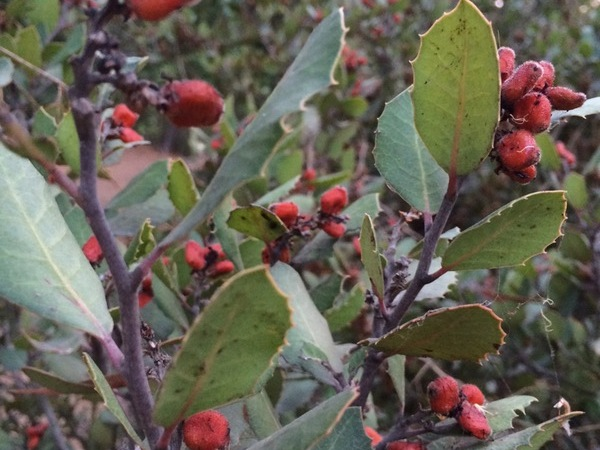
\includegraphics[height=3.05cm]{plant.jpg}\\[1.4mm]
      \accenttext{分布外图像}\\[.6mm]
      \small 植物不在类别清单里，选猫或狗都会出错。
    \end{column}
  \end{columns}
  \par\vspace{3.5mm}
  \accenttext{分布外检测}帮助分类器发现超出已知类别的图像，并回答“未知”。
  \note{55 秒。先请大家设想，手机相册只设了猫和狗两类。指向狗的照片，问它该放进哪一类。再看植物，给它贴哪个现有标签都会错。这时，相册能回答“未知”就够了。这里的“未知”取决于任务给定的类别。如果相册本来就有植物这一类，同一张照片就属于已知范围。
    \par \paperref{4}{两张示例照片取自原论文图 2。}}
\end{frame}

\section{激活与评分}

\begin{frame}[t]{看图前选好的负标签，到了测试时有用吗？}
  \pdfbookmark[3]{01:20　预选负标签的问题}{timing-80}
  \small NegLabel 在看图前挑选词义远离已知类名的词作负标签。“植物”和“轮船”都与猫狗相去甚远，可遇到植物照片时，这两个词的用处很不一样。
  \par\vspace{1.4mm}
  \begin{columns}[T,onlytextwidth]
    \begin{column}{.48\linewidth}\centering
      \accenttext{多数预选词很少匹配测试图像}\\[.8mm]
      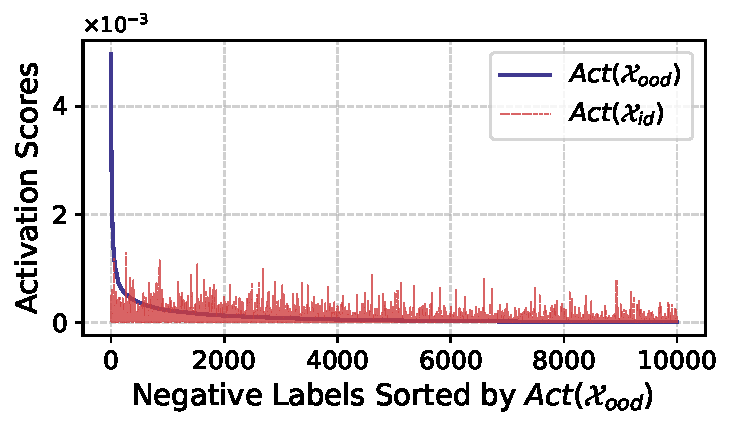
\includegraphics[width=\linewidth,height=2.88cm,keepaspectratio]{fig1a-activation.pdf}
      \par\raggedright\small 激活 $\Act(\mathcal X)$ 是词在图像集 $\mathcal X$ 上的平均匹配概率。蓝线为 Places 场景集 $\mathcal X_{\rm ood}$，红线为 ImageNet 已知类图像集 $\mathcal X_{\rm id}$。
    \end{column}
    \begin{column}{.49\linewidth}\centering
      \accenttext{加入更多词，误报反而可能增加}\\[.8mm]
      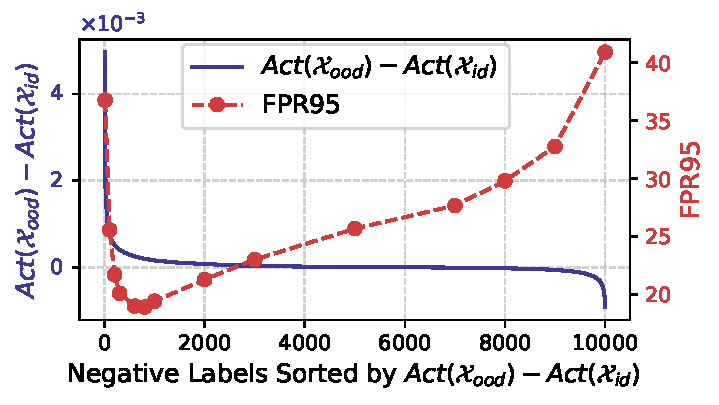
\includegraphics[width=\linewidth,height=2.88cm,keepaspectratio]{fig1b-fpr95.pdf}
      \par\raggedright\small 按 OOD 减 ID 的激活差（蓝线）给词排序。加入排在后面的词，误报率（红线）回升。
    \end{column}
  \end{columns}
  \vspace{1.7mm}
  \small 两图横轴均为词的排名，激活轴以千分之一为单位。右图红线读右轴（\%）。\accenttext{FPR95} 是检出 95\% 正例时的负例误报率，越低越好。
  \note{50 秒。静态方法先挑词，让它们与已知类名竞争。一个词分到的概率由已知类和候选词一起归一化得到。指向左图拖得很长的尾部。许多词虽然离已知类名很远，却几乎匹配不上测试照片。再看右图红线，越过低点继续加词，误报反而回升。能不能让眼前的照片帮我们挑词？
    \par \paperref{2}{原论文图 1(a)、(b)}\quad · \quad\paperref{3}{NegLabel 如何预选负标签并计算图像的 ID 分数。}}
\end{frame}

\begin{frame}[t,label=paper-overview]{TANL 的整体思路}
  \pdfbookmark[3]{02:10　TANL 的整体思路}{timing-130}
  \begin{columns}[c,onlytextwidth]
    \begin{column}{.31\linewidth}\centering
      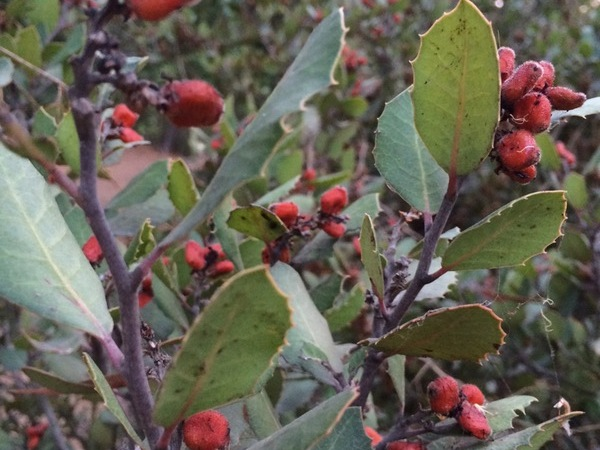
\includegraphics[width=\linewidth]{plant.jpg}
      \par\vspace{1.2mm}\small 假设猫狗相册里最近\par
      出现了许多植物照片。
    \end{column}
    \begin{column}{.64\linewidth}
      \accenttext{从最近的照片里找两组参照}\par
      \small 模型挑出自己较有把握的照片，一组看起来像猫狗，另一组看起来不像。
      \par\vspace{2.3mm}
      \normalsize\accenttext{挑出能区分两组的词}\par
      \small 如果“植物”常匹配疑似未知的照片，很少匹配那些像猫狗的照片，它就是有用的负标签。
      \par\vspace{2.3mm}
      \normalsize\accenttext{用这些词判断新照片}\par
      \small 越能区分两组的词，影响越大。如果“植物”比猫狗类名更匹配新照片，模型就更倾向于回答“未知”。
    \end{column}
  \end{columns}
  \par\vspace{3.8mm}
  新的测试图像陆续到来，模型会重新选词。整个过程无需人工标注或重新训练。
  \note{50 秒。接着看那张植物照片。测试时没有人告诉模型哪些照片是植物，它只能先挑出一些自己有把握的例子。如果“植物”经常匹配那些看起来不像猫狗的照片，很少匹配猫狗，这个词就值得用来判断新照片。如果后来出现很多船只照片，有用的词也会变。下一页再解释，模型怎样在没有真实标签的情况下得到这两组参照。
    \par \paperref{4}{原论文第 3.3 节与图 2}\quad · \quad\paperref{5}{测试时选词与评分。} 猫狗相册为讲解用的假设情景。}
\end{frame}

\begin{frame}[t]{没有测试真值时，用高置信图像估计两组响应}
  \pdfbookmark[3]{03:00　正负队列与本批估计}{timing-180}
  \begin{columns}[T,onlytextwidth]
    \begin{column}{.60\linewidth}
      \lead{从测试流中找两组代理样本}
      \small 初步 ID 分数衡量图像有多像已知类。高分图进正队列 $\mathcal X_{\pos}$，低分图进负队列 $\mathcal X_{\negq}$，中间的跳过。两侧分别用类名文本和噪声图像初始化，各按先进先出（FIFO）保留最近入队的 300 个特征。
      \par\vspace{2.5mm}
      \accenttext{把本批也算进去}\quad\small 上标 $b$ 表示当前批次。$\mathcal X^b_{\pos}$ 和 $\mathcal X^b_{\negq}$ 是本批筛出的两组。每侧分别按历史 95\%、本批 5\% 融合平均响应。
    \end{column}
    \begin{column}{.365\linewidth}
      \lead{纹理图像激活了哪些词？}
      \par\vspace{1.5mm}
      \begin{minipage}[c]{.42\linewidth}
        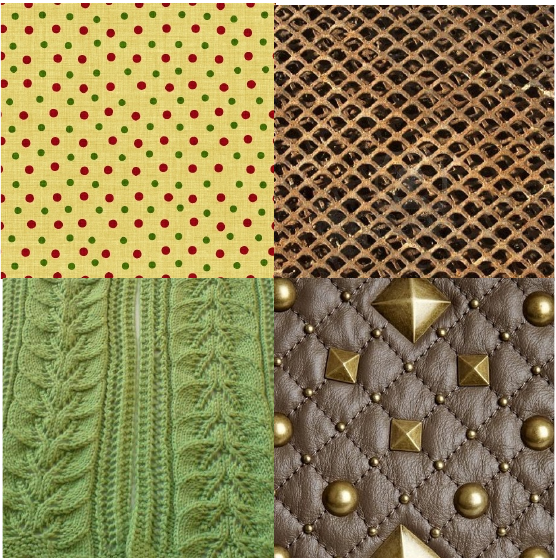
\includegraphics[width=\linewidth]{fig4-textures.png}
      \end{minipage}\hfill
      \begin{minipage}[c]{.55\linewidth}\small
        \textbf{grating}（格栅）\\$+0.0022$\\[1.8mm]
        \textbf{polka dot}（圆点）\\$+0.0018$
      \end{minipage}
      \par\vspace{2.0mm}\small 正值表示该词在疑似 OOD 图像上的平均响应更强。
    \end{column}
  \end{columns}
  \par\vspace{3mm}
  \small 对一个候选词 $y$，将融合后的负侧响应减去正侧响应，得到本批估计的激活差 $\widehat{\Act}_b(y)$。按差值从大到小选词。
  \note{75 秒。分数高和低分别代表更像已知类和更像未知类，中间区域先跳过。冷启动时，正队列用类名文本特征，负队列用噪声图像特征。测试图陆续替换这些初值。对每个候选词，先在同一候选词库上归一化，再分别估计正负两侧的平均概率。本批某侧没有高置信样本时只用那侧的历史。用右边格栅与圆点的例子解释一个正的激活差。
    \par \paperref{4}{候选词的平均激活与正负队列的更新}\quad · \quad\paperref{5}{如何融合历史队列与当前批次的激活来选词}\quad · \quad\paperref{8}{图 4 的 Textures 示例。}}
\end{frame}

\begin{frame}[t]{排在前面的负标签，会影响更多次评分}
  \pdfbookmark[3]{04:15　前缀评分算例}{timing-255}
  \small 待测图像 $\mathbf x$ 的单位向量为 $\mathbf v$，第 $i$ 个已知类的文本单位向量为 $\mathbf t_i$。\\
  将入选的 $M$ 个负标签按估计激活差降序排列，第 $j$ 个负标签的文本单位向量为 $\widetilde{\mathbf t}_j$。
  \par\vspace{1.6mm}
  \begin{columns}[T,onlytextwidth]
    \begin{column}{.48\linewidth}\centering
      \accenttext{全部 $C$ 个已知类的总响应}\par\vspace{.6mm}
      $\displaystyle A=\sum_{i=1}^{C}
        \exp\!\left(\frac{\mathbf v\cdot\mathbf t_i}{\tau}\right)$\par
    \end{column}
    \begin{column}{.465\linewidth}\centering
      \accenttext{排名前 $m$ 个负标签的总响应}\par\vspace{.6mm}
      $\displaystyle B_m=\sum_{j=1}^{m}
        \exp\!\left(\frac{\mathbf v\cdot\widetilde{\mathbf t}_j}{\tau}\right)$\par
    \end{column}
  \end{columns}
  \par\vspace{1.6mm}
  \small 点积（$\cdot$）即余弦相似度，$\tau$ 为正温度。$\exp$ 取指数得到未归一化响应，$\sum$ 将响应相加。
  \par\vspace{2mm}
  \begin{columns}[T,onlytextwidth]
    \begin{column}{.48\linewidth}
      \accenttext{对各前缀的已知类份额取平均}\par\vspace{.7mm}
      $\displaystyle \Saa(\mathbf x)=\frac{1}{M}
         \sum_{m=1}^{M}\frac{A}{A+B_m}$\par\vspace{1mm}
      \small 前 $m$ 个负词构成一个前缀。$\Saa$ 是图像的 ID 分数，首词进入全部 $M$ 个分母。
    \end{column}
    \begin{column}{.465\linewidth}
      \accenttext{两个已知类、两个负标签的例子}\par
      \small 猫、狗的响应相加为 $A=2+4=6$。
      \par\vspace{.6mm}
      \begin{tabular*}{\linewidth}{@{\extracolsep{\fill}}lr@{}}
        $B_1=6$     & $6/(6+6)=0.50$\\
        $B_2=6+3=9$ & $6/(6+9)=0.40$\\
        \midrule
        两个份额的平均 & $\mathbf{0.45}$\\
      \end{tabular*}
    \end{column}
  \end{columns}
  \note{80 秒。固定一张图，看它和每个标签分别有多像。单位向量的点积给出余弦相似度。论文写图文匹配概率时省略了温度缩放。这里把每个相似度除以同一个正温度，再取指数、求和。猫和狗都算进已知类总响应，所以分子始终是六。负侧先只算第一个词，下一次再加第二个词。两个已知类份额分别为零点五和零点四，平均为零点四五。负词的顺序由两组图像上的估计激活差决定，而这里相加的是每个词对眼前这张图的响应。
    \par \paperref{3}{图文匹配概率、已知类总概率与温度缩放}\quad · \quad\paperref{5}{逐个加入负词后，如何对已知类的概率份额取平均。}}
\end{frame}

\section{流程与结果}

\begin{frame}[t]{把筛样本、选词和评分连成一个测试批次}
  \pdfbookmark[3]{05:35　完整测试流程}{timing-335}
  \begin{columns}[c,onlytextwidth]
    \begin{column}{.65\linewidth}\centering
      \begin{tikzpicture}
        \node[anchor=south west,inner sep=0] (fig) at (0,0)
          {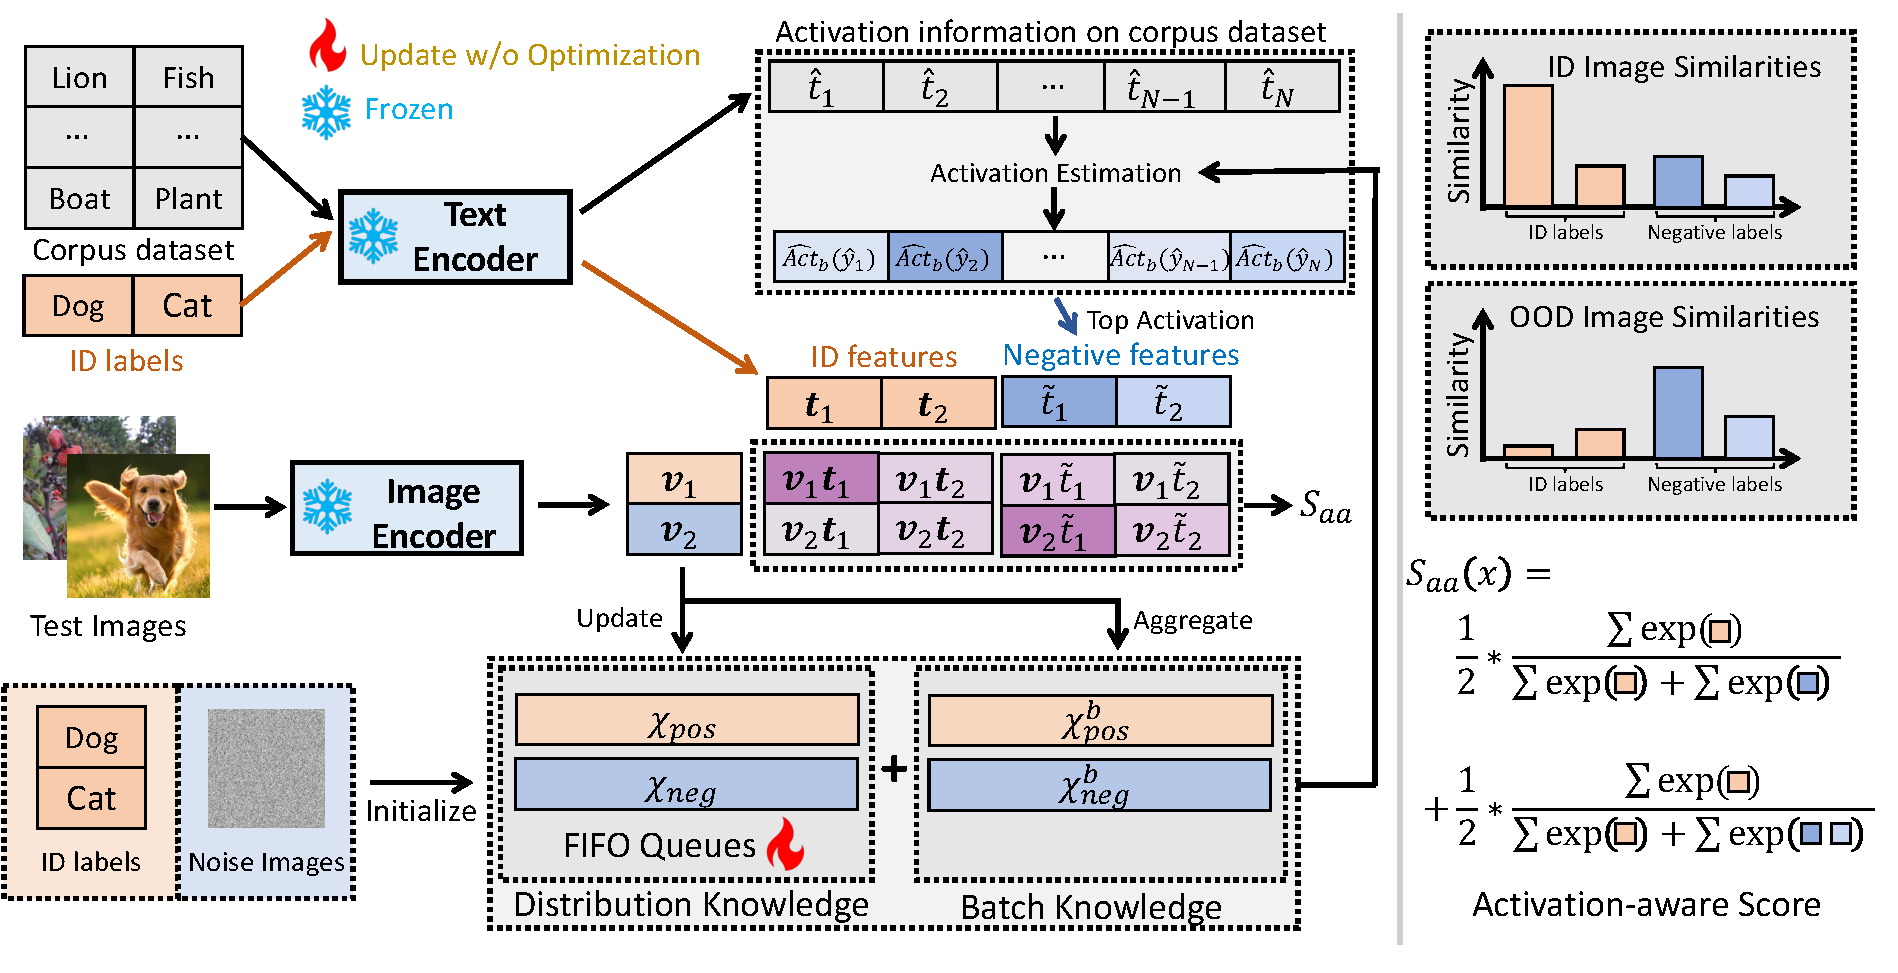
\includegraphics[width=\linewidth]{fig2-framework.pdf}};
        \begin{scope}[x={(fig.south east)},y={(fig.north west)},
          draw=peaking,line width=1.4pt,rounded corners=1pt]
          \begin{ocg}{Sample screening}{screen}{1}
            \draw (.25,.02) rectangle (.69,.30);
          \end{ocg}
          \begin{ocg}{Label selection}{rank}{0}
            \draw (.39,.68) rectangle (.73,.99);
          \end{ocg}
          \begin{ocg}{Scoring}{score}{0}
            \draw (.74,.02) rectangle (.995,.99);
          \end{ocg}
        \end{scope}
      \end{tikzpicture}
    \end{column}
    \begin{column}{.32\linewidth}\small
      \actionsocg{}{screen}{rank score}{\accenttext{1\quad 筛样本}}\par
      $\mathbf v_1,\mathbf v_2$ 是两张图的向量。用已有状态筛出本批高置信样本。\par\vspace{1.8mm}
      \actionsocg{}{rank}{screen score}{\accenttext{2\quad 选负词}}\par
      在 $N$ 个候选词中，按估计激活差选前 $M$ 个。\par\vspace{1.8mm}
      \actionsocg{}{score}{screen rank}{\accenttext{3\quad 给图评分}}\par
      用 $\Saa$ 判断是否拒识，再把高置信样本写回队列。
    \end{column}
  \end{columns}
  \vspace{1.4mm}
  \small 图中下标是编号。$\widehat y_k,\widehat{\mathbf t}_k$ 是第 $k$ 个候选词及其文本向量，$\mathbf t_i$ 和 $\widetilde{\mathbf t}_j$ 是第 $i$ 个已知类（橙色）和第 $j$ 个入选负词（蓝色）的文本向量。中央的 $\mathbf v_1\mathbf t_1$ 表示图文向量的内积。
  \par 雪花表示编码器冻结，火焰表示免训练更新。点击右侧步骤标题可切换高亮。
  \note{65 秒。用原论文的图串起刚才的思路，依次点击右侧三个步骤。下方用队列中的历史图像和本批有把握的图像作参照。上方比较两组对每个词的响应，重新选词。右侧用前缀平均给每张图打分，低分拒识。高置信样本随后进入队列，供下一批使用。
    \par \paperref{4}{原论文图 2}\quad · \quad\paperref{5}{算法 1}。橙色为已知类，蓝色为负词。雪花表示冻结，火焰表示免训练更新。点击步骤标题可切换高亮。}
\end{frame}

\begin{frame}[t]{动态选词降低了误报，改变到达顺序也会改变结果}
  \pdfbookmark[3]{06:40　论文结果与顺序敏感性}{timing-400}
  \small 原论文用 ImageNet 的 1,000 个已知类，冻结 CLIP 的 ViT-B/16 图像编码器（基础型视觉 Transformer，图像块为 $16\times16$ 像素）。表中结果取 iNaturalist、SUN、Places 和 Textures 四组 OOD 的平均值。
  \par\vspace{1mm}\small AUROC 是受试者工作特征曲线下面积，衡量整体排序能力。表内均为百分数，$\downarrow$ 越低越好，$\uparrow$ 越高越好。
  \par\vspace{2.3mm}
  \begin{columns}[T,onlytextwidth]
    \begin{column}{.485\linewidth}
      \lead{同一测试设置下换方法}
      \par\vspace{1.4mm}\small
      \begin{tabular*}{\linewidth}{@{\extracolsep{\fill}}lrr@{}}
        \toprule
        方法 & FPR95 $\downarrow$ & AUROC $\uparrow$\\\midrule
        静态 NegLabel &25.40&94.21\\
        动态 TANL &\textbf{9.81}&\textbf{97.97}\\\bottomrule
      \end{tabular*}
    \end{column}
    \begin{column}{.465\linewidth}
      \lead{固定 TANL，只换测试顺序}
      \par\vspace{1.4mm}\small
      \begin{tabular*}{\linewidth}{@{\extracolsep{\fill}}lr@{}}
        \toprule
        到达顺序 & FPR95 $\downarrow$\\\midrule
        ID 与 OOD 随机混排 &9.81\\
        全部 ID 先到 &16.47\\
        全部 OOD 先到 &16.73\\\bottomrule
      \end{tabular*}
    \end{column}
  \end{columns}
  \par\vspace{2.5mm}
  \small \accenttext{小组从队列入手}\quad 如果很少有真实 ID 进入正队列，下一批还能据此选对负词吗？
  \note{80 秒。左边只读两行对照，误报率从二十五点四降到九点八一，整体排序也改善了。右边固定同一方法和数据，先来哪类图像就足以改变误报率，说明队列里的历史样本有影响。交接时把问题留给第二部分。我们在另一个基准上实际数了多少样本进入正队列。
    \par \paperref{6}{原论文表 1}\quad · \quad\paperref{18}{附录表 A16}。四组 OOD 为 iNaturalist、SUN、Places 和 Textures。}
\end{frame}
